\documentclass[12pt,aspectratio=43]{beamer}

% 自訂字體的封包
\usepackage{fontspec}

% 導入圖形與表格的封包
\usepackage{graphicx}
\graphicspath{{./20251210_Meeting}}

\usepackage{booktabs}

% 排列多個子圖形的封包
\usepackage{subfigure} 

 % 提供進階數學環境與公式排版
\usepackage{mathtools, amsmath, amsfonts, amsthm, latexsym} 

%% 設定中文字體
\usepackage{xeCJK}
\setCJKmainfont[AutoFakeBold=3.5 , AutoFakeSlant=0.2]{標楷體}
\setmainfont{Times New Roman}
\XeTeXlinebreaklocale "zh"
\XeTeXlinebreakskip = 0pt plus 1pt

% 自訂字體顏色的封包
\usepackage{color} 

% 圖表自動編號的封包
\usepackage{caption} 

% 允許表格的一格能多列呈現的封包
\usepackage{multirow} 

% 可指定表格排版的封包
\usepackage{array}

% 翻轉表格的封包
\usepackage{lscape} 

% 序列標號
\usepackage{enumerate} 

%% 設定自動編號
\setbeamertemplate{caption}[numbered]

%% 自訂顏色
\definecolor{Myblue}{RGB}{57,108,144}
\definecolor{Default_Blue}{RGB}{52,51,171}

% (動畫)字會若隱若現的顯示
\beamersetuncovermixins{\opaqueness<1->{45}}{\opaqueness<1->{95}} 

% 設定中文的標籤
\renewcommand{\figurename}{圖} 
\renewcommand{\tablename}{表} 

% 排版形式 
\mode<presentation>{
\usetheme{Berlin}
% enumerate 及 item 的形狀
\setbeamertemplate{itemize items}[triangle]
% 調整外框形式的字體大小
\setbeamerfont{headline}{size=\scriptsize}
\setbeamerfont{footline}{size=\scriptsize}
% 取消右下方的跳轉工具列
\setbeamertemplate{navigation symbols}{} 
% 自定義2：清除外框下緣但僅出頁碼
\setbeamertemplate{footline}[page number] 
% 顏色主題
\usecolortheme{dove}
% 設定頁面邊界
\setbeamersize{text margin left=0.6cm, text margin right=0.6cm}
\special{papersize=\the\paperwidth,\the\paperheight}
\providecommand{\tabularnewline}{\\}
}

\title{Meeting 1210}
\author{黃丞暘}
\institute{國立東華大學應數統計所}
\date{December 10, 2025}

\begin{document}

% 封面
\begin{frame}
  \titlepage
\end{frame}

% 目錄
\begin{frame}{\textbf{Index}}
  \tableofcontents
\end{frame}

% DISCUSSION 
\section{12.03 Discussion}

\begin{frame}{\textbf{12.03 Discussion}}
\linespread{1.5}
  Semiconductor Manufacturing Process
  \begin{itemize}
    \item Given the fitted model $y=\hat{f}$
    \begin{enumerate}[]
      \item Describe what $hat{f}$ is when $x$ belongs to neighbors of $X_0$ for some “interesting” $X_0$

    \end{enumerate}
  \end{itemize}
  \begin{itemize}
    \item 研究  $\hat f(x),\quad x \in \mathcal{N}(X_0)$ 以理解模型在局部的解釋性、結構。
    \begin{enumerate}[]
      \item 建構 \(\hat f\) 的方法（回歸或機器學習），使用鄰近資料 \((y_k, x_k)\) 建立局部模型
    \end{enumerate}

  \end{itemize}
\end{frame}

% TO DO
\section{12.03 Todo}

\begin{frame}{\textbf{12.03 Todo}}
\linespread{1.5}
  \begin{itemize}[]
    \item Do the SMOTE before PCA after delete outliers
  \end{itemize}
  \begin{itemize}[]
    \item Decide a $x_k$(p dimension) from neighbors of $X_0$ to do the regression
  \begin{enumerate}[]

    \item 在每個 cluster 抽幾個代表點 X₀，例如：

1. cluster center（在 PCA 空間的重心，找最近的樣本）

2. y=1 且預測機率高的點

3. 預測錯誤的點（不穩定區）
  \end{enumerate}

  \end{itemize}
\end{frame}

% 結果
\section{Resulut - What I do this time}

\begin{frame}{\textbf{Results I}　{SMOTE + PCA + KMeans}}
\linespread{0.9}

\begin{center}
  \begin{minipage}{0.45\linewidth}
    \centering
    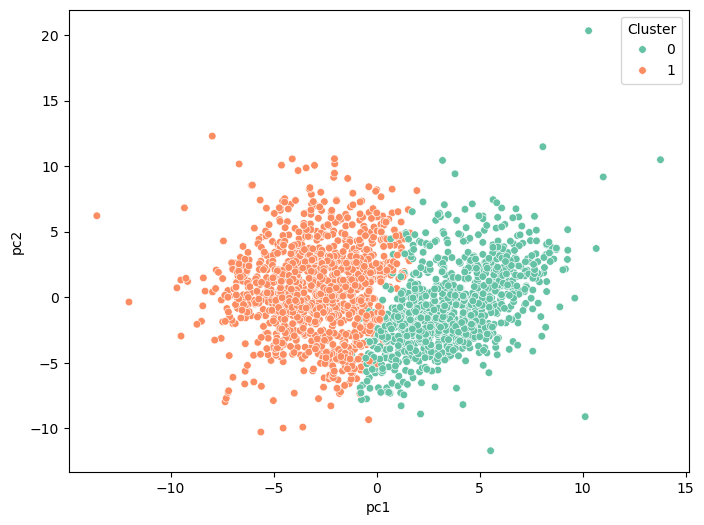
\includegraphics[width=\linewidth]{pca.png}
  \end{minipage}
  \hspace{0.3em}
  \begin{minipage}{0.45\linewidth}
    \centering
    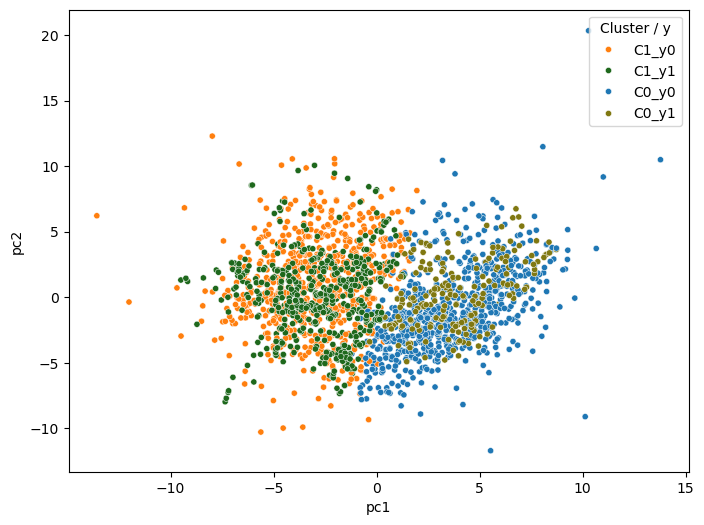
\includegraphics[width=\linewidth]{pca2.png}
  \end{minipage}
\end{center}

\small{$$
\begin{array}{c|cc}
\text{cluster} & 0 & 1 \\
\hline
y=0 & 743 & 687 \\
y=1 & 205 & 510 \\
\end{array}
$$}

\end{frame}

\begin{frame}{\textbf{Results I}　{5-folds cv - mean}}
\linespread{0.9}

{\small
$$
\begin{array}{l|ccc}
\text{model} 
& \text{ACC} & \text{FAR} & \text{ROCAU}\\
\hline
\text{LR}  & 0.8520 & 0.1011 & 0.5459\\
\text{SVM} & 0.9304 & 0.0041 & 0.5027\\
\text{DT}  & 0.8149 & 0.1415 & 0.5309\\
\text{RF}  & 0.9304 & 0.0048 & 0.5074\\
\text{XGB} & 0.9272 & 0.0096 & 0.5145\\
\end{array}
$$
}

{\small
$$
\begin{array}{l|ccc|ccc}
\text{model} 
& \text{$C_0$ACC} & \text{$C_0$FAR} & \text{$C_0$ROCAU} 
& \text{$C_1$ACC} & \text{$C_1$FAR} & \text{$C_1$ROCAU}\\
\hline
\text{LR}  & *0.9219 & *0.0942 & *0.9431 & *0.9131 & 0.1456 & *0.9233\\
\text{SVM} & *0.9895 & *0.0013 & *0.9774 & *0.9883 & 0.0044 & *0.9870\\
\text{DT}  & *0.9114 & *0.0686 & *0.8852 & *0.8622 & 0.1716 & *0.8681\\
\text{RF}  & *0.9631 & 0.0000 & *0.9146 & *0.9749 & *0.0014 & *0.9708\\
\text{XGB} & *0.9799 & 0.0000 & *0.9537 & *0.9741 & 0.0248 & *0.9739\\
\end{array}
$$
}
\end{frame}

% --- 結束 ---
\section*{結束}

\begin{frame}[plain] % 產生無外框的頁面
	\begin{center}
		{\Huge The End}
		\bigskip\bigskip 

		{\LARGE Questions  \&  Comments}
	\end{center}
\end{frame}
\end{document}ㄒ
